\documentclass[11pt,a4paper]{article}

\usepackage[utf8]{inputenc}
\usepackage[T1]{fontenc}
\usepackage[margin=1in]{geometry}
\usepackage[table]{xcolor}
\usepackage[most]{tcolorbox}
\usepackage{hyperref}
\usepackage{tabularx}
\usepackage{booktabs}
\usepackage{tikz}
\usepackage{fancyhdr}
\usepackage{fontawesome5}
\usepackage{amsmath}
\usepackage{graphicx}
\usepackage{float}

% --- Premium Typography & Spacing ---
\usepackage{mathpazo}
\usepackage{setspace}
\setstretch{1.15}

% --- Premium Section Headings ---
\usepackage{titlesec}
\titleformat{\section}
  {\normalfont\Large\bfseries\color{dpiblue}}{\thesection}{1em}{}[{\color{dpicloud}\vspace{0.2cm}\titlerule[1pt]}]
\titleformat{\subsection}
  {\normalfont\large\bfseries\color{dpiteal}}{\thesubsection}{1em}{}

% --- Premium Hyperlinks ---
\hypersetup{
    colorlinks=true,
    linkcolor=dpiblue,
    filecolor=dpiblue,      
    urlcolor=dpiteal,
    citecolor=dpiblue
}

% Custom Header Style
\pagestyle{fancy}
\setlength{\headheight}{25pt}
\fancyhf{}
\fancyhead[L]{\raisebox{-0.2\height}{
\includegraphics[height=15pt]{logo.png}}\hspace{0.2cm}\textbf{\color{dpiblue} DPI-LS Framework}}
\fancyhead[R]{\color{dpiblue} Measuring Validation (V)}
\fancyfoot[C]{\color{dpiblue}\textbf{Page \thepage}}
\renewcommand{\headrulewidth}{1pt}
\renewcommand{\headrule}{\hbox to\headwidth{\color{dpiblue}\leaders\hrule height \headrulewidth\hfill}}
\usetikzlibrary{shapes.geometric, arrows.meta, positioning, calc, backgrounds, fit, trees, mindmap, matrix, shadows}

% Define DPI-LS Brand Colors
\definecolor{dpiblue}{HTML}{2b3a67}
\definecolor{dpigreen}{HTML}{498467}
\definecolor{dpired}{HTML}{b0413e}
\definecolor{dpilight}{HTML}{e5f9e0}
\definecolor{dpicloud}{HTML}{f4a261}
\definecolor{dpiteal}{HTML}{318281}

% Define Custom GitHub-Style Alerts
\newtcolorbox{dpinote}[1][]{enhanced, colback=blue!5!white, colframe=dpiblue, title={\textbf{\faInfoCircle\ NOTE}}, fonttitle=\bfseries, attach boxed title to top left={xshift=5mm,yshift=-2mm}, #1}
\newtcolorbox{dpiimportant}[1][]{enhanced, colback=red!5!white, colframe=dpired, title={\textbf{\faExclamationTriangle\ IMPORTANT}}, fonttitle=\bfseries, attach boxed title to top left={xshift=5mm,yshift=-2mm}, #1}
\newtcolorbox{dpitip}[1][]{enhanced, colback=dpigreen!5!white, colframe=dpigreen, boxrule=0.5pt, leftrule=3pt, sharp corners, #1}

\begin{document}

\begin{titlepage}
    \pagecolor{dpiblue}
    \color{white}
    \begin{center}
        \vspace*{1.5cm}
        
\includegraphics[width=6cm]{logo.png} \\[1.5cm]
        
        {\Huge \textbf{Measuring Validation}} \\[0.7cm]
        {\LARGE \textbf{Guide for the DPI-LS Project}}
        
        \vspace{2cm}
        
        {\color{dpicloud}\rule{0.5\textwidth}{1.5pt}}
        
        \vspace{2cm}
        
        {\Large \textit{Digital Performance Index --- Validation Dimension (V)}} \\[1cm]
        
        {\large Structural Compliance, Deterministic Outputs \& Pipeline Integration}
        
        \vfill
        
        % Stylish Geometric Cover Overlay
        \begin{tikzpicture}[remember picture, overlay]
            \fill[white, opacity=0.05] (current page.north east) circle (5cm);
            \fill[white, opacity=0.05] (current page.south west) circle (7cm);
            \fill[dpiteal, opacity=0.1] (current page.south east) circle (9cm);
            
            % Giant faded icon in the center as a watermark
            \node[font=\fontsize{150}{150}\selectfont, text=white, opacity=0.03] at (current page.center) {\faFileCode};
        \end{tikzpicture}
        
        \renewcommand{\arraystretch}{1.3}
        \begin{tabular}{rl}
            \textbf{Framework:} & Digital Performance Index (DPI-LS) \\
            \textbf{Dimension:} & Validation (V) --- Weight: 10\% \\
            \textbf{Version:} & 1.0 (Extended Enterprise Edition) \\
            \textbf{Status:} & Architectural Reference \\
        \end{tabular}
        
        \vspace{2cm}
        
        {\color{dpicloud}\rule{0.5\textwidth}{1pt}} \\[0.5cm]
        
        {\large DPI-LS Architecture Team}
        
        \vspace{0.3cm}
        {\normalsize Document Developed by \textbf{Malkapurapu Sivamanikanta}}
        
        \vspace*{1cm}
    \end{center}
\end{titlepage}
\pagecolor{white}
\color{black}

\tableofcontents
\newpage

% ---------------------------------------------------------
% 1. EXECUTIVE SUMMARY & INTRODUCTION
% ---------------------------------------------------------
\section{Executive Summary \& Introduction}

\begin{dpinote}
The \textbf{Digital Performance Index (DPI-LS)} framework quantifies AI agent performance across 7 distinct dimensions. Within this framework, the \textbf{Validation (V)} dimension tracks an agent's ability to produce deterministic, structured, and machine-readable outputs.
\end{dpinote}

Autonomous AI Agents exist within complex enterprise pipelines. If an agent is tasked with extracting financial metrics and writes a beautiful, poetic paragraph summarizing the data, but fails to format that data as a required JSON array, \textbf{the pipeline breaks}. The downstream database cannot ingest poetry; it requires deterministic schema compliance.

The Validation ($V$) dimension specifically measures this structural obedience. It does not judge the \textit{factual correctness} of the output (which is evaluated by Quality $Q$), but rather the \textit{architectural formatting} of the payload. Did the agent return JSON? Did it use the `<answer>` XML tags? Did it format its data using Markdown tables `| col | col |`?

Because structural failures instantly crash autonomous orchestration workflows, the Validation dimension acts as a critical \textbf{Compliance Gate}. If an agent fails to consistently validate its structural requirements, the DPI-LS Engine violently caps the agent's overall composite score, preventing structural anomalies from hiding behind high productivity.

\vspace{0.5cm}
\hrule
\vspace{1cm}

% ---------------------------------------------------------
% 2. VALIDATION STRATEGY MIND MAP
% ---------------------------------------------------------
\section{Validation Strategy Mind Map}

The following mind map defines the core pillars of AI Agent Validation monitored within the DPI-LS framework.

\vspace{1cm}
\begin{center}
\resizebox{0.9\textwidth}{!}{
\begin{tikzpicture}[
  mindmap,
  every node/.style={concept, execute at begin node=\hskip0pt, drop shadow},
  root concept/.append style={concept color=dpiblue, fill=dpiblue, line width=1ex, text=white, font=\large\bfseries},
  level 1 concept/.append style={font=\small\bfseries, level distance=5.5cm, text=white},
  level 2 concept/.append style={font=\footnotesize, level distance=3.5cm, text=black},
  grow cyclic
]

\node[root concept] {AI Agent \\ Validation}
  child[concept color=dpicloud, sibling angle=90] { node {Schema \\ Compliance}
    child[sibling angle=55] { node[fill=white] {JSON \\ Objects} }
    child[sibling angle=55] { node[fill=white] {JSON \\ Arrays} }
    child[sibling angle=55] { node[fill=white] {Pydantic \\ Maps} }
  }
  child[concept color=dpiteal, sibling angle=90] { node {Semantic \\ Tagging}
    child[sibling angle=55] { node[fill=white] {XML \\ Tags} }
    child[sibling angle=55] { node[fill=white] {<answer> \\ Blocks} }
    child[sibling angle=55] { node[fill=white] {<result> \\ Blocks} }
  }
  child[concept color=dpigreen, sibling angle=90] { node {Markdown \\ Formatting}
    child[sibling angle=55] { node[fill=white] {\#\# Section \\ Headers} }
    child[sibling angle=55] { node[fill=white] {| Markdown \\ Tables |} }
    child[sibling angle=55] { node[fill=white] {Code \\ Fences} }
  }
  child[concept color=dpired, sibling angle=90] { node {The Hard \\ Gate}
    child[sibling angle=55] { node[fill=white] {$< 0.60$ \\ Trigger} }
    child[sibling angle=55] { node[fill=white] {Needs \\ Optimization} }
    child[sibling angle=55] { node[fill=white] {Unsafe \\ Flag} }
  };
\end{tikzpicture}
}
\end{center}

\newpage

% ---------------------------------------------------------
% 3. THE MATHEMATICS OF VALIDATION
% ---------------------------------------------------------
\section{The Mathematics of Validation}

The Validation dimension provides a normalized fractional score indicating how often the agent adhered to structural schema rules. Validation carries a weighting of \textbf{10\% (0.10)} on the final composite DPI-LS score.

\begin{dpiimportant}
\textbf{Formula:} $V = \frac{\text{Validated Components}}{\text{Total Required Components}}$
\end{dpiimportant}

\begin{itemize}
    \item \textbf{\color{dpiblue}\faCheckCircle\ Validated Components:} The raw integer of components correctly detected by the engine's `\_looks\_structured()` heuristics (e.g., finding the exact Markdown table requested).
    \item \textbf{\color{dpiteal}\faListUl\ Total Required Components:} The baseline integer of structural formats the enterprise system explicitly required the agent to output for the given batch.
\end{itemize}

\subsection{The Vacuous Safe Default}

Unlike humans, autonomous systems do not always require strict formatting rules. Some conversational agents are simply designed to chat. If an agent is assigned $0$ required structural components, calculating the $V$ ratio ($0 / 0$) would result in a mathematically undefined `DivisionByZero` error.

To solve this, the DPI-LS Engine utilizes a \textbf{Vacuous Default}. 

If $\text{Total Required Components} = 0$, the engine automatically defaults the score to $V = \mathbf{1.0}$. 
\begin{quote}
\textit{``An agent cannot be penalized for failing to validate a structure that was never asked of it.'' - DPI-LS Core Design Philosophy}
\end{quote}
This allows new agents with undefined schemas to coast safely at a perfect 1.0 until actual validation requirements are enforced by the FinOps or DevOps teams.

\subsection{The 0.60 Hard Compliance Gate}

While $10\%$ weight might seem small, the Validation dimension possesses a catastrophic override switch known as a \textbf{Hard Compliance Gate}.

If an agent fails to follow formatting rules and its $V$ score drops below $\mathbf{0.60}$ ($60\%$), it triggers the DPI-LS Compliance Gate. 
\begin{itemize}
    \item \textbf{Rule 1:} The agent's overall DPI-LS composite score is violently capped at exactly \textbf{69} (the top of the ``Needs Optimization'' band).
    \item \textbf{Rule 2:} The agent is flagged with an \texttt{unsafe=True} telemetry marker.
\end{itemize}

Even if an agent is hyper-productive ($P=1.0$), perfectly cheap ($C=1.0$), and logically flawless ($Q=1.0$), failing to format its data breaks the enterprise CI/CD pipeline. The 69 cap accurately reflects this critical operational hazard.

\newpage

% ---------------------------------------------------------
% 4. MATHEMATICAL MASTERCLASS
% ---------------------------------------------------------
\section{Mathematical Masterclass: End-to-End Score Calculation}

The following masterclass walks through the exact end-to-end mathematical pipeline used by the DPI-LS engine to calculate an agent's final Validation score. We break this down into 4 comprehensive phases.

\vspace{0.5cm}

% ---------------- PHASE 1 ----------------
\subsection{Phase 1: Define Required Components}

The Enterprise Data Engineering team requires an agent to scrape a financial database and return the results in a highly structured format so that downstream Python scripts can ingest it.

\begin{tcolorbox}[enhanced, colback=dpicloud!5!white, colframe=dpiblue, title={\textbf{Phase 1: Enterprise Schema Requirements}}, fonttitle=\bfseries]
For this batch run, the agent is tasked to produce a specific set of outputs. The orchestrator explicitly requires the following components:
\begin{itemize}
    \item \textbf{Requirement 1:} A JSON Array wrapping the entire payload (\texttt{[ \{ \} ]}).
    \item \textbf{Requirement 2:} Markdown Table formatting for the raw statistics (\texttt{| col | col |}).
    \item \textbf{Requirement 3:} A Markdown Sub-header (\texttt{\#\# Financial Summary}).
    \item \textbf{Requirement 4:} XML Semantic Tags wrapping the final recommendation (\texttt{<answer> BUY </answer>}).
    \item \textbf{Requirement 5:} Another Markdown Sub-header (\texttt{\#\# Risk Profile}).
\end{itemize}
\textbf{Total Required Components ($Req$):} $\mathbf{5}$
\end{tcolorbox}

\newpage

% ---------------- PHASE 2 ----------------
\subsection{Phase 2: Agent Telemetry Capture}

The agent executes the run and passes the raw text output into the `dpi\_ls` observability collector. The engine's `\_looks\_structured()` deterministic regex scanner reads the raw text to hunt for structural adherence.

\begin{tcolorbox}[enhanced, colback=dpicloud!5!white, colframe=dpiteal, title={\textbf{Phase 2: The Structure Scanner (`\_looks\_structured`)}}, fonttitle=\bfseries]
The engine scans the string and detects the following markers:
\vspace{0.2cm}
\begin{itemize}
    \item \faCheckCircle\ \textbf{Scan Pass:} Engine detects \texttt{\{ "financials": ... \}} (JSON object format matched).
    \item \faCheckCircle\ \textbf{Scan Pass:} Engine detects \texttt{| Quarter | Revenue |} (Markdown Table format matched).
    \item \faCheckCircle\ \textbf{Scan Pass:} Engine detects \texttt{\#\# Financial Summary} (Markdown Header matched).
    \item \faTimesCircle\ \textbf{Scan Fail:} Engine detects "I recommend BUY" (Failed to use \texttt{<answer>} XML tags).
    \item \faTimesCircle\ \textbf{Scan Fail:} Engine detects "Risk Profile:" (Failed to use \texttt{\#\#} Markdown headers).
\end{itemize}

\vspace{0.2cm}
\textbf{Final Validated Components ($Val$):} $\mathbf{3}$
\end{tcolorbox}

\newpage

% ---------------- PHASE 3 ----------------
\subsection{Phase 3: The Ratio Calculation}

We now have the raw mathematical integers required for the Validation formula.

\begin{tcolorbox}[enhanced, colback=orange!5!white, colframe=orange, title={\textbf{Phase 3: Calculating $V$}}, fonttitle=\bfseries]
The engine calculates the base ratio:
\[
V = \frac{\text{Validated Components}}{\text{Total Required Components}} = \frac{3}{5} = \mathbf{0.60}
\]
\textbf{Business Meaning:} The agent was $60\%$ compliant with the data engineering team's schema requirements. It dropped the ball on the XML tags and the second markdown header, forcing human engineers to manually format the text.
\end{tcolorbox}

\vspace{0.5cm}

% ---------------- PHASE 4 ----------------
\subsection{Phase 4: Bounding and Gate Trigger}

Because the $V$ score is exactly $0.60$, we must check the Hard Compliance Gate logic.

\begin{tcolorbox}[enhanced, colback=dpigreen!5!white, colframe=dpigreen, title={\textbf{Phase 4: The Hard Gate Evaluation}}, fonttitle=\bfseries]
The DPI-LS Engine evaluates the $V$ score against the critical threshold:
\[
\text{Gate Limit: } V < 0.60 \implies \text{Trigger Cap}
\]
Since our agent scored exactly $0.60$, it mathematically survives the gate evaluation ($0.60 \not< 0.60$). 

\vspace{0.2cm}
\textbf{Final Masterclass Conclusion:} \\
The agent successfully processed 3 out of the 5 required structural schemas. Because it hit a $60\%$ validation rate, it barely scraped by the Hard Compliance Gate. The agent earns a final Validation dimension score of \textbf{0.60 (60\%)}. Its composite DPI-LS score is allowed to remain organic, avoiding the aggressive `69` Needs Optimization penalty cap!
\end{tcolorbox}

\newpage

% ---------------------------------------------------------
% 5. THE FINAL V-SCORE CALCULATION FLOW
% ---------------------------------------------------------
\subsection{The Final V-Score Calculation Flow}

The diagram below illustrates the horizontal mathematical flow of data to calculate the final $V$ score, matching the exact 4-phase mathematical masterclass example.

\vspace{1cm}
\begin{center}
\resizebox{1.0\textwidth}{!}{
\begin{tikzpicture}[
    node distance=1.0cm and 0.5cm,
    incident/.style={rectangle, draw=dpiblue, fill=dpicloud!20, thick, text width=2.8cm, align=center, minimum height=1cm, rounded corners},
    critical/.style={rectangle, draw=orange, fill=orange!10, thick, text width=2.8cm, align=center, minimum height=1cm, rounded corners},
    gate/.style={rectangle, draw=dpired, fill=dpired!10, thick, text width=2.8cm, align=center, minimum height=1cm, rounded corners},
    arrow/.style={-{Stealth[scale=1.2]}, thick, dpiblue},
    result/.style={rectangle, draw=dpigreen, fill=dpilight, thick, text width=3.5cm, align=center, minimum height=1.5cm, rounded corners, drop shadow}
]

% Row 1: The Raw Input
\node[incident] (req_comp) {Required\\$Req = 5$};
\node[incident, right=1.5cm of req_comp] (val_comp) {Validated\\$Val = 3$};
\node[critical, right=1.5cm of val_comp] (ratio) {Ratio\\$3 / 5 = 0.60$};

% Row 2: Bounding and Gate
\node[gate, below=1cm of ratio] (hard_gate) {Compliance Gate\\$0.60 \geq 0.60$ (Pass)};
\node[result, left=2cm of hard_gate] (final) {\textbf{Final V-Score}\\\Large \textbf{0.60}};

% Arrows Layer 1
\draw[arrow] (req_comp) -- (val_comp);
\draw[arrow] (val_comp) -- (ratio);

% Downward Arrows
\draw[arrow] (ratio) -- (hard_gate);

% Final Row Arrows
\draw[arrow] (hard_gate) -- (final);

\end{tikzpicture}
}
\end{center}
\vspace{1cm}

\newpage

% ---------------------------------------------------------
% 6. INTEGRATION ARCHITECTURE
% ---------------------------------------------------------
\section{Integration Architecture}

The beauty of the Validation dimension is that it is purely deterministic. Unlike Quality ($Q$), which requires an expensive LLM as a judge to evaluate factual accuracy, Validation is evaluated natively in Python without hitting the network.

When an agent calls `dpi\_ls.monitor()`, the engine intercepts the raw text output. It runs the lightweight `\_looks\_structured()` parser over the prose. 

\begin{figure}[H]
    \centering
    \begin{tikzpicture}[
        node distance=2cm,
        box/.style={rectangle, draw=dpiblue, fill=dpicloud!10, thick, text width=3cm, align=center, minimum height=1.5cm, rounded corners},
        codebox/.style={rectangle, draw=dpiteal, fill=dpiteal!10, thick, text width=4cm, align=center, minimum height=1.5cm, rounded corners},
        arrow/.style={-{Stealth[scale=1.2]}, thick, dpiblue}
    ]
    
    \node[box] (agent) {Agent Run};
    \node[codebox, right=of agent] (prose) {Raw Output Text\\(\textit{"Here is your data..."})};
    \node[box, right=of prose] (parser) {`\_looks\_structured()`\\Regex Engine};
    \node[codebox, below=1.5cm of parser] (score) {Validation Metrics\\($Val$ / $Req$)};
    \node[box, left=of score] (db) {SQLite DB\\`dpi\_ls.db`};
    
    \draw[arrow] (agent) -- (prose);
    \draw[arrow] (prose) -- (parser);
    \draw[arrow] (parser) -- (score);
    \draw[arrow] (score) -- (db);
    
    \end{tikzpicture}
    \caption{Deterministic Validation Pipeline Architecture}
\end{figure}

By moving structure validation into the observability collector rather than relying on another LLM prompt, the DPI-LS framework ensures lightning-fast execution and zero-hallucination metric collection.

\vspace{0.5cm}

% ---------------------------------------------------------
% 7. TELEMETRY & PATTERN DETECTION LOGIC
% ---------------------------------------------------------
\section{Telemetry \& Pattern Detection Logic}

The DPI-LS Engine searches for specific structural patterns to increment the Validated Components ($Val$) counter.

\renewcommand{\arraystretch}{1.5}
\begin{table}[H]
    \centering
    \begin{tabularx}{\textwidth}{|>{\bfseries\color{dpiblue}}l|X|X|}
    \hline
    \rowcolor{dpicloud!20}
    \textbf{Component Type} & \textbf{Detection Logic} & \textbf{Example} \\
    \hline
    JSON Object & Parses string for strict key-value braces & \texttt{\{ "name": "AI" \}} \\
    \hline
    JSON Array & Parses string for strict object brackets & \texttt{[ \{"id": 1\} ]} \\
    \hline
    XML Tag & Regex match for bounded semantic wrappers & \texttt{<answer> True </answer>} \\
    \hline
    Markdown Header & Matches \texttt{\#\#} or \texttt{\#\#\#} leading markers & \texttt{\#\# Analysis Summary} \\
    \hline
    Markdown Table & Regex match for bar delimiters \texttt{|} & \texttt{| Name | Age |} \\
    \hline
    Code Fences & Matches triple backticks \texttt{```json} & \texttt{```json \textbackslash{}n \{\} ```} \\
    \hline
    \end{tabularx}
    \caption{DPI-LS Structural Detection Mapping}
\end{table}

\vspace{0.5cm}

% ---------------------------------------------------------
% 8. TELEMETRY & INTEGRATIONS
% ---------------------------------------------------------
\section{Telemetry \& Integrations}

Validation data must be sourced directly from the orchestration engine and parsing framework to prevent agents from hallucinating their own success metrics. The table below outlines how common enterprise systems map to the DPI-LS Validation parameters.

\vspace{0.5cm}
\begin{table}[H]
\centering
\renewcommand{\arraystretch}{1.4}
\rowcolors{2}{gray!10}{white}
\arrayrulecolor{gray!50}
\begin{tabularx}{\textwidth}{| >{\raggedright\arraybackslash}X >{\raggedright\arraybackslash}X >{\raggedright\arraybackslash}p{3.5cm} >{\raggedright\arraybackslash}X |}
\hline
\rowcolor{dpiblue} \textcolor{white}{\textbf{Validation Data}} & \textcolor{white}{\textbf{What It Measures}} & \textcolor{white}{\textbf{Source System}} & \textcolor{white}{\textbf{Actual Data Comes From}} \\
\hline
Schema Definitions & The required JSON/XML formats & TypeChat / JSON Schema & Schema Registry API \\
JSON Compliance & If the string strictly parses as JSON & Guardrails AI & Guardrails Logs \\
XML Adherence & If the XML/HTML tags are perfectly nested & Outlines / Guidance & Outlines Exceptions \\
Markdown Headers & Presence of \texttt{\#\#} tags & Langfuse & Langfuse Scores \\
Semantic Tags & Bounding blocks like \texttt{<answer>} & TruEra / TruLens & TruLens Evaluator \\
Pydantic Validation & Strict type checking for agent outputs & Instructor / Marvin & \texttt{ValidationError} Traces \\
Graph State Adherence & Does output match the state machine edge? & LangSmith & LangSmith State Traces \\
Missing Keys & Which specific JSON keys were dropped & BAML (Boundary ML) & BAML Telemetry \\
Orchestrator Requires & Baseline number of requested schemas & Portkey / Helicone & Gateway Payload Logs \\
Failure Tracking & Which specific schemas failed & Datadog LLM & Datadog APM Spans \\
\hline
\end{tabularx}
\end{table}
\vspace{0.5cm}

\vspace{1cm}

% ---------------------------------------------------------
% 9. VALIDATION TELEMETRY CONTRACT
% ---------------------------------------------------------
\section{Validation Telemetry Contract}

The DPI-LS framework uses the strictly typed \texttt{ValidationStats} block inside the Pydantic contract (\texttt{contract/models.py}) to map these validation metrics.

\vspace{0.5cm}
\begin{center}
\renewcommand{\arraystretch}{1.5}
\begin{tabularx}{\textwidth}{@{} l l c X @{}}
\toprule
\rowcolor{dpiblue} 
\textcolor{white}{\textbf{Contract Field}} & \textcolor{white}{\textbf{Python Type}} & \textcolor{white}{\textbf{Default}} & \textcolor{white}{\textbf{Description \& Role}} \\
\midrule
\texttt{required\_components} & \texttt{int} & $0$ & Total components the orchestrator requires. \\
\rowcolor{dpilight}
\texttt{validated\_components} & \texttt{int} & $0$ & Count of components that passed the \texttt{\_looks\_structured()} scan. \\
\texttt{is\_json\_compliant} & \texttt{bool} & False & True if the final payload strictly parses as JSON. \\
\rowcolor{dpilight}
\texttt{failed\_schemas} & \texttt{list[str]} & \texttt{[]} & Array of expected schemas the agent failed to generate. \\
\bottomrule
\end{tabularx}
\end{center}
\vspace{0.5cm}

% ---------------------------------------------------------
% 9. REAL-WORLD BUSINESS SCENARIOS
% ---------------------------------------------------------
\section{Real-World Business Scenarios}

\begin{tcolorbox}[enhanced, colback=dpilight, colframe=dpigreen, title={\textbf{Scenario 1: The Prose Trap}}, fonttitle=\bfseries]
\textbf{Situation:} A customer support agent is asked to analyze a refund request and return the JSON object: \texttt{\{"refund\_approved": true\}}. Instead, the agent is overly helpful and writes: \textit{"I have reviewed the request. Yes, the refund is approved! Here is your JSON: \texttt{\{"refund\_approved": true\}}"}.

\textbf{Outcome:} Because the agent hallucinated conversational prose outside of the required strict JSON schema, the `\_looks\_structured()` parser fails to parse the full string as a valid object. Validation drops, reflecting the fact that this "helpful" prose just crashed the downstream API webhook.
\end{tcolorbox}

\begin{tcolorbox}[enhanced, colback=blue!5!white, colframe=dpiblue, title={\textbf{Scenario 2: The Vacuous Start}}, fonttitle=\bfseries]
\textbf{Situation:} A developer launches a brand new conversational chatbot using \texttt{dpi\_ls.monitor()}. There are no required tables, JSON blobs, or XML tags. The agent just talks to the user.

\textbf{Outcome:} The engine assigns a requirement baseline of $0$. Applying the Vacuous Default rule, the agent is granted a Validation score of $1.0$ (100\%). It is not penalized for failing to write schemas it was never asked for.
\end{tcolorbox}

\begin{tcolorbox}[enhanced, colback=red!5!white, colframe=dpired, title={\textbf{Scenario 3: The Hard Gate Trigger}}, fonttitle=\bfseries]
\textbf{Situation:} A complex agent swarm is scoring $98\%$ in Execution, $95\%$ in Quality, and $100\%$ in Cost. However, it was asked to provide 10 markdown tables but only provided 4. Its Validation score is $4/10 = \mathbf{0.40}$.

\textbf{Outcome:} Because $0.40$ falls below the $0.60$ threshold, the Hard Compliance Gate fires. The agent's composite score plummets from a massive 95 down to the hard cap of \textbf{69 (Needs Optimization)}. The dashboard flags the agent as `Unsafe` because an agent that refuses to format data cannot be trusted in production.
\end{tcolorbox}

\newpage

% ---------------------------------------------------------
% 10. CONCLUSION & NEXT STEPS
% ---------------------------------------------------------
\section{Conclusion \& Next Steps}

\begin{tcolorbox}[enhanced, colback=gray!5!white, colframe=dpiblue, boxrule=1pt, arc=0mm, drop shadow, top=5mm, bottom=5mm]
\begin{center}
\textbf{\large \textcolor{dpiblue}{The Validation Dimension Guarantees}}\\
\textbf{\large \textcolor{dpiblue}{Structural System Compliance}}
\end{center}
\vspace{0.3cm}
\begin{center}
\begin{tikzpicture}[remember picture, overlay]
\node[text=dpiblue, opacity=0.08, font=\fontsize{60}{60}\selectfont] at (0, 0.5) {\faFileCode};
\end{tikzpicture}
The Validation dimension ensures that an agent produces deterministic, structured payloads. By violently capping the composite score if Validation drops below $0.60$, the DPI-LS framework guarantees that dangerous, unparseable conversational prose does not crash critical enterprise data pipelines.
\end{center}
\end{tcolorbox}



\subsection{Next Steps Roadmap}

\begin{center}
\resizebox{0.9\textwidth}{!}{
\begin{tikzpicture}[
    node distance=1cm,
    step1/.style={rectangle, draw=dpiblue, fill=dpiblue!5, thick, text width=3.5cm, align=center, minimum height=2.5cm, rounded corners, drop shadow},
    step2/.style={rectangle, draw=dpiteal, fill=dpiteal!5, thick, text width=3.5cm, align=center, minimum height=2.5cm, rounded corners, drop shadow},
    step3/.style={rectangle, draw=dpigreen, fill=dpigreen!5, thick, text width=3.5cm, align=center, minimum height=2.5cm, rounded corners, drop shadow},
    arrow/.style={-{Stealth[scale=1.5]}, thick, dpicloud}
]

\node[step1] (s1) {\textcolor{dpiblue}{\Large\faDatabase}\\[0.2cm]\textcolor{dpiblue}{\textbf{Step 1}}\\[0.2cm]\small Map Enterprise Schema Requirements};
\node[step2, right=of s1] (s2) {\textcolor{dpiteal}{\Large\faRobot}\\[0.2cm]\textcolor{dpiteal}{\textbf{Step 2}}\\[0.2cm]\small Deploy \texttt{\_looks\_structured()} Scanners};
\node[step3, right=of s2] (s3) {\textcolor{dpigreen}{\Large\faChartLine}\\[0.2cm]\textcolor{dpigreen}{\textbf{Step 3}}\\[0.2cm]\small Automate Compliance Gate Triggers};

\draw[arrow] (s1) -- (s2);
\draw[arrow] (s2) -- (s3);

% Timeline bar underneath
\draw[line width=3pt, dpiblue] ([yshift=-0.2cm, xshift=-1cm]s1.south west) -- ([yshift=-0.2cm]s1.south);
\draw[line width=3pt, dpiteal] ([yshift=-0.2cm]s1.south) -- ([yshift=-0.2cm]s2.south);
\draw[line width=3pt, dpigreen] ([yshift=-0.2cm]s2.south) -- ([yshift=-0.2cm, xshift=1cm]s3.south east);

\node[circle, fill=dpiblue, text=white, inner sep=1.5pt, font=\tiny\bfseries] at ([yshift=-0.2cm]s1.south) {1};
\node[circle, fill=dpiteal, text=white, inner sep=1.5pt, font=\tiny\bfseries] at ([yshift=-0.2cm]s2.south) {2};
\node[circle, fill=dpigreen, text=white, inner sep=1.5pt, font=\tiny\bfseries] at ([yshift=-0.2cm]s3.south) {3};

\node[below=0.3cm of s1, text=dpiblue] {Now};
\node[below=0.3cm of s2, text=dpiteal] {Near-term};
\node[below=0.3cm of s3, text=dpigreen] {Q-end};

\end{tikzpicture}
}
\end{center}

\vspace{1cm}
\begin{tcolorbox}[enhanced, colback=dpiblue, colframe=dpiblue, boxrule=0pt, arc=2mm]
\begin{center}
\textcolor{white}{\textbf{\Large Document Developed By}}\\[0.15cm]
\textcolor{white}{\textbf{\Large AI Team}}\\[0.15cm]
\textcolor{white}{\textbf{\Large Malkapurapu Sivamanikanta}}\\[0.3cm]
\textcolor{dpicloud}{\small Digital Performance Index --- Validation Dimension (V) --- Version 1.0}\\[0.1cm]
\textcolor{dpicloud}{\small Architectural Reference $\bullet$ Confidential}
\end{center}
\end{tcolorbox}

\end{document}
